\documentclass[
  doc,
  longtable,
  nolmodern,
  notxfonts,
  notimes,
  mask,
  colorlinks=true,linkcolor=blue,citecolor=blue,urlcolor=blue]{apa7}

\usepackage{amsmath}
\usepackage{amssymb}

\geometry{inner=1in, outer=1in}
\fancyhfoffset[LE,RO]{0cm}



\RequirePackage{longtable}
\RequirePackage{threeparttablex}

\makeatletter
\renewcommand{\paragraph}{\@startsection{paragraph}{4}{\parindent}%
	{0\baselineskip \@plus 0.2ex \@minus 0.2ex}%
	{-.5em}%
	{\normalfont\normalsize\bfseries\typesectitle}}

\renewcommand{\subparagraph}[1]{\@startsection{subparagraph}{5}{0.5em}%
	{0\baselineskip \@plus 0.2ex \@minus 0.2ex}%
	{-\z@\relax}%
	{\normalfont\normalsize\bfseries\itshape\hspace{\parindent}{#1}\textit{\addperi}}{\relax}}
\makeatother




\usepackage{longtable, booktabs, multirow, multicol, colortbl, hhline, caption, array, float, xpatch}
\usepackage{subcaption}


\renewcommand\thesubfigure{\Alph{subfigure}}
\setcounter{topnumber}{2}
\setcounter{bottomnumber}{2}
\setcounter{totalnumber}{4}
\renewcommand{\topfraction}{0.85}
\renewcommand{\bottomfraction}{0.85}
\renewcommand{\textfraction}{0.15}
\renewcommand{\floatpagefraction}{0.7}

\usepackage{tcolorbox}
\tcbuselibrary{listings,theorems, breakable, skins}
\usepackage{fontawesome5}

\definecolor{quarto-callout-color}{HTML}{909090}
\definecolor{quarto-callout-note-color}{HTML}{0758E5}
\definecolor{quarto-callout-important-color}{HTML}{CC1914}
\definecolor{quarto-callout-warning-color}{HTML}{EB9113}
\definecolor{quarto-callout-tip-color}{HTML}{00A047}
\definecolor{quarto-callout-caution-color}{HTML}{FC5300}
\definecolor{quarto-callout-color-frame}{HTML}{ACACAC}
\definecolor{quarto-callout-note-color-frame}{HTML}{4582EC}
\definecolor{quarto-callout-important-color-frame}{HTML}{D9534F}
\definecolor{quarto-callout-warning-color-frame}{HTML}{F0AD4E}
\definecolor{quarto-callout-tip-color-frame}{HTML}{02B875}
\definecolor{quarto-callout-caution-color-frame}{HTML}{FD7E14}

%\newlength\Oldarrayrulewidth
%\newlength\Oldtabcolsep


\usepackage{hyperref}




\providecommand{\tightlist}{%
  \setlength{\itemsep}{0pt}\setlength{\parskip}{0pt}}
\usepackage{longtable,booktabs,array}
\usepackage{calc} % for calculating minipage widths
% Correct order of tables after \paragraph or \subparagraph
\usepackage{etoolbox}
\makeatletter
\patchcmd\longtable{\par}{\if@noskipsec\mbox{}\fi\par}{}{}
\makeatother
% Allow footnotes in longtable head/foot
\IfFileExists{footnotehyper.sty}{\usepackage{footnotehyper}}{\usepackage{footnote}}
\makesavenoteenv{longtable}

\usepackage{graphicx}
\makeatletter
\newsavebox\pandoc@box
\newcommand*\pandocbounded[1]{% scales image to fit in text height/width
  \sbox\pandoc@box{#1}%
  \Gscale@div\@tempa{\textheight}{\dimexpr\ht\pandoc@box+\dp\pandoc@box\relax}%
  \Gscale@div\@tempb{\linewidth}{\wd\pandoc@box}%
  \ifdim\@tempb\p@<\@tempa\p@\let\@tempa\@tempb\fi% select the smaller of both
  \ifdim\@tempa\p@<\p@\scalebox{\@tempa}{\usebox\pandoc@box}%
  \else\usebox{\pandoc@box}%
  \fi%
}
% Set default figure placement to htbp
\def\fps@figure{htbp}
\makeatother







\usepackage{newtx}

\defaultfontfeatures{Scale=MatchLowercase}
\defaultfontfeatures[\rmfamily]{Ligatures=TeX,Scale=1}





\title{Volunteer Report Cité-Unis}


\shorttitle{Cité-Unis}


\usepackage{etoolbox}






\author{Jan Pfänder}



\affiliation{
{Paris}}




\leftheader{Pfänder}



\abstract{This report analyzes surveys for four different cohorts of
Cité-Unis volunteers who did their service civique (2020-2024). }



\authornote{ 

\par{       }
\par{Correspondence concerning this article should be addressed to Jan
Pfänder, Email: \href{mailto:janlukas.pfaender@gmail.com}{janlukas.pfaender@gmail.com}}
}

\makeatletter
\let\endoldlt\endlongtable
\def\endlongtable{
\hline
\endoldlt
}
\makeatother

\urlstyle{same}



\usepackage{booktabs}
\usepackage{longtable}
\usepackage{array}
\usepackage{multirow}
\usepackage{wrapfig}
\usepackage{float}
\usepackage{colortbl}
\usepackage{pdflscape}
\usepackage{tabu}
\usepackage{threeparttable}
\usepackage{threeparttablex}
\usepackage[normalem]{ulem}
\usepackage{makecell}
\usepackage{xcolor}
\makeatletter
\@ifpackageloaded{caption}{}{\usepackage{caption}}
\AtBeginDocument{%
\ifdefined\contentsname
  \renewcommand*\contentsname{Table of contents}
\else
  \newcommand\contentsname{Table of contents}
\fi
\ifdefined\listfigurename
  \renewcommand*\listfigurename{List of Figures}
\else
  \newcommand\listfigurename{List of Figures}
\fi
\ifdefined\listtablename
  \renewcommand*\listtablename{List of Tables}
\else
  \newcommand\listtablename{List of Tables}
\fi
\ifdefined\figurename
  \renewcommand*\figurename{Figure}
\else
  \newcommand\figurename{Figure}
\fi
\ifdefined\tablename
  \renewcommand*\tablename{Table}
\else
  \newcommand\tablename{Table}
\fi
}
\@ifpackageloaded{float}{}{\usepackage{float}}
\floatstyle{ruled}
\@ifundefined{c@chapter}{\newfloat{codelisting}{h}{lop}}{\newfloat{codelisting}{h}{lop}[chapter]}
\floatname{codelisting}{Listing}
\newcommand*\listoflistings{\listof{codelisting}{List of Listings}}
\makeatother
\makeatletter
\makeatother
\makeatletter
\@ifpackageloaded{caption}{}{\usepackage{caption}}
\@ifpackageloaded{subcaption}{}{\usepackage{subcaption}}
\makeatother

% From https://tex.stackexchange.com/a/645996/211326
%%% apa7 doesn't want to add appendix section titles in the toc
%%% let's make it do it
\makeatletter
\xpatchcmd{\appendix}
  {\par}
  {\addcontentsline{toc}{section}{\@currentlabelname}\par}
  {}{}
\makeatother

%% Disable longtable counter
%% https://tex.stackexchange.com/a/248395/211326

\usepackage{etoolbox}

\makeatletter
\patchcmd{\LT@caption}
  {\bgroup}
  {\bgroup\global\LTpatch@captiontrue}
  {}{}
\patchcmd{\longtable}
  {\par}
  {\par\global\LTpatch@captionfalse}
  {}{}
\apptocmd{\endlongtable}
  {\ifLTpatch@caption\else\addtocounter{table}{-1}\fi}
  {}{}
\newif\ifLTpatch@caption
\makeatother

\begin{document}

\maketitle




\setlength\LTleft{0pt}




\section{Introduction}\label{introduction}

In this report, we address three main questions regarding volunteers who
do there service civique in France:

\begin{enumerate}
\def\labelenumi{\arabic{enumi}.}
\tightlist
\item
  Who are the volunteers? (Section~\ref{sec-who})
\item
  How does the service civique change the volunteers' attitudes and
  views? (Section~\ref{sec-within-change})
\item
  Are there trends between different cohorts of volunteers?
  (Section~\ref{sec-between-change})
\item
  What predicts whether volunteers\ldots{}
\end{enumerate}

\begin{itemize}
\tightlist
\item
  \ldots end their contract early? (Section~\ref{sec-rupture})
\item
  \ldots are more satisfied ? (Section~\ref{sec-satisfaction})
\item
  \ldots are more confident about their future?
  (Section~\ref{sec-perception-avenir})
\end{itemize}

\begin{enumerate}
\def\labelenumi{\arabic{enumi}.}
\setcounter{enumi}{4}
\tightlist
\item
  How do volunteers differ between the different programs?
\end{enumerate}

\begin{itemize}
\tightlist
\item
  Ciné (Section~\ref{sec-cine})
\item
  Ecology (Section~\ref{sec-ecovolonterre})
\end{itemize}

We rely on questionnaires collected by Cité-Unis for four different
cohorts of volunteers who did their service civique for a year
(2020-2021; 2021-2022; 2022-2023; 2023-2024). These questionnaires are
very extensive. For the present analyses, we selected a subset of key
questions (a full list can be found in the
\href{codebook.qmd}{codebook}). Note that this selection of variables
was based only on the questionnaire of the first cohort (2020/21). As a
result, potentially interesting variables that only appear in later
questionnaires will not appear here.

\section{Who are the volunteers ?}\label{sec-who}

Here, we just review some demographic variables briefly. An extensive
summary table with sample demographics across the different cohorts can
be found in \href{tables.qmd}{Tables}.

\subsection{Geographic location}\label{geographic-location}

Volunteers came from 80 different departments (see
Figure~\ref{fig-map-repartition}). On average, across the different
cohorts, most volunteers came from Bouches-du-Rhône (n = 404), followed
by Nord (n = 350) and Seine-Saint-Denis (n = 316).

Overall, there has been a steady increase in volunteers, from 6386 in
20-21 to 7848 in 23-24, and an average increase of 490.4 per year. Since
the 20-21 cohort, each departement has on average increased by 26.7.
There were 51 departements who saw an increase, and 14 who saw a
decrease (see Figure~\ref{fig-map-trend}). For details on the trend of
each departement, see \href{tables.qmd}{Tables}.

\begin{figure}

\caption{\label{fig-map-repartition}Répartition des volontaires en
France à travers le temps.}

\centering{

\pandocbounded{\includegraphics[keepaspectratio]{index_files/figure-pdf/fig-map-repartition-1.pdf}}

}

\end{figure}%

\begin{figure}

\caption{\label{fig-map-trend}Evolution de recrutement pour la promo de
2023-24 par rapport à 2020-21.}

\centering{

\pandocbounded{\includegraphics[keepaspectratio]{index_files/figure-pdf/fig-map-trend-1.pdf}}

}

\end{figure}%

\subsection{Age}\label{age}

Across all promos, the majority of volunteers is between 18 and 20 years
old (Figure~\ref{fig-age}).

\begin{figure}

\caption{\label{fig-age}Number of volunteers per age group, within the
different promos. Note that in the percentage plot, the percentages are
relative to all volunteers from the respective promo.}

\begin{minipage}{0.50\linewidth}

\subcaption{\label{fig-age-1}(absolute numbers)}

\centering{

\pandocbounded{\includegraphics[keepaspectratio]{index_files/figure-pdf/fig-age-1.pdf}}

}

\end{minipage}%
%
\begin{minipage}{0.50\linewidth}

\subcaption{\label{fig-age-2}(percentages)}

\centering{

\pandocbounded{\includegraphics[keepaspectratio]{index_files/figure-pdf/fig-age-2.pdf}}

}

\end{minipage}%

\end{figure}%

\subsection{Education}\label{education}

As shown in Figure~\ref{fig-education}, volunteers with a ``Bac + 3 et
plus'' are relatively rare. The share of volunteers with a ``Bac à Bac +
2'' has been constantly decreasing, from 48\% in 2020/21 to 40\% in
2023/24. By contrast, volunteers ``Infra-bac'', have been increasing
from 32\% in 2020/21 to 43\% in 2023/24.

\begin{figure}

\caption{\label{fig-education}Number of volunteers per education level,
within the different promos. Note that in the percentage plot, the
percentages are relative to all volunteers from the respective promo.}

\begin{minipage}{0.50\linewidth}

\subcaption{\label{fig-education-1}(absolute numbers)}

\centering{

\pandocbounded{\includegraphics[keepaspectratio]{index_files/figure-pdf/fig-education-1.pdf}}

}

\end{minipage}%
%
\begin{minipage}{0.50\linewidth}

\subcaption{\label{fig-education-2}(percentages)}

\centering{

\pandocbounded{\includegraphics[keepaspectratio]{index_files/figure-pdf/fig-education-2.pdf}}

}

\end{minipage}%

\end{figure}%

\subsection{Sex}\label{sex}

There is a relatively stable difference regarding sex, with more women
(\textasciitilde60\%) being volunteers than men (Figure~\ref{fig-sex}).

\begin{figure}

\caption{\label{fig-sex}Number of male and female volunteers, within the
different promos. Note that in the percentage plot, the percentages are
relative to all volunteers from the respective promo.}

\begin{minipage}{0.50\linewidth}

\subcaption{\label{fig-sex-1}(absolute numbers)}

\centering{

\pandocbounded{\includegraphics[keepaspectratio]{index_files/figure-pdf/fig-sex-1.pdf}}

}

\end{minipage}%
%
\begin{minipage}{0.50\linewidth}

\subcaption{\label{fig-sex-2}(percentages)}

\centering{

\pandocbounded{\includegraphics[keepaspectratio]{index_files/figure-pdf/fig-sex-2.pdf}}

}

\end{minipage}%

\end{figure}%

\section{How have volunteers changed their
attitudes?}\label{sec-within-change}

First, this analysis is restricted by attrition, i.e.~volunteers
dropping out of the surveys over time (see Figure~\ref{fig-attrition}).
Second, there are only two questions that volunteers of the same promo
have been asked at different time points: {[}REPORT them here{]}.

\begin{figure}

\caption{\label{fig-attrition}Number of volunteers per survey time
point. Volunteers who appear under `q0' have participated in the program
but have not even filled out the first questionnaire. Note that in the
percentage plot, the percentages are relative to all volunteers from the
respective promo.}

\begin{minipage}{0.50\linewidth}

\subcaption{\label{fig-attrition-1}(absolute numbers)}

\centering{

\pandocbounded{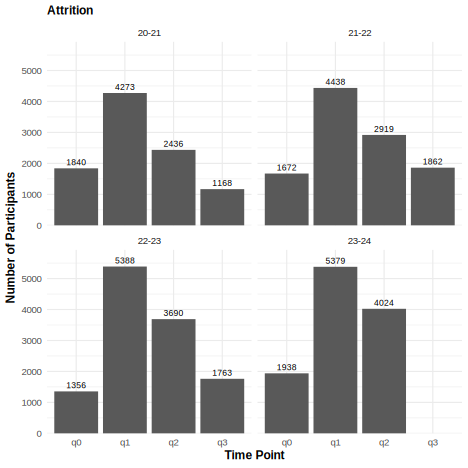
\includegraphics[keepaspectratio]{index_files/figure-pdf/fig-attrition-1.pdf}}

}

\end{minipage}%
%
\begin{minipage}{0.50\linewidth}

\subcaption{\label{fig-attrition-2}(percentages)}

\centering{

\pandocbounded{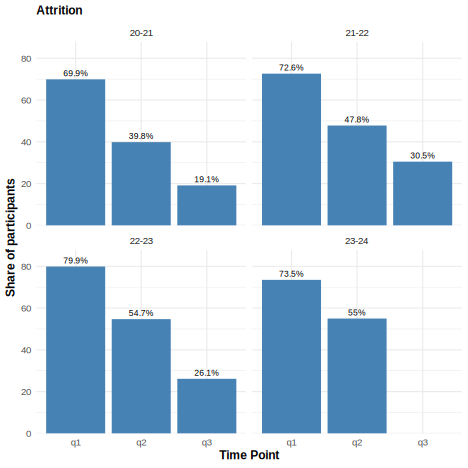
\includegraphics[keepaspectratio]{index_files/figure-pdf/fig-attrition-2.pdf}}

}

\end{minipage}%

\end{figure}%

\subsection{Voting}\label{voting}

The figures in this section shows all volunteers who answered the
question {[}XX{]} at both time points (q1 and q2), with either ``yes''
or ``no'', for the different promos (promo 2020-21,
Figure~\ref{fig-vote_derniers_elections-2020}; promo 2021-22,
Figure~\ref{fig-vote_derniers_elections-2021}; 2022-23,
Figure~\ref{fig-vote_derniers_elections-2022}; 2023-24,
Figure~\ref{fig-vote_derniers_elections-2023}).

This descriptive analysis suggests that the service civique did not have
an impact on voting behavior, on average. However, this analysis is
pooled across different cohorts, not all of which would have had the
chance to change their voting behavior during their year volunteering,
simply because there were no elections.

\subsubsection{Promo 2020-21}\label{promo-2020-21}

\begin{figure}

\caption{\label{fig-vote_derniers_elections-2020}Promo 2020-21. Change
in volunteers reporting whether they voted or not during the last
elections, between Q1 and Q2. Note that this analysis considers only
answers of volunteers who answered either yes or no at \emph{both} time
points.}

\begin{minipage}{0.50\linewidth}

\subcaption{\label{fig-vote_derniers_elections-2020-1}Alluvial plot}

\centering{

\pandocbounded{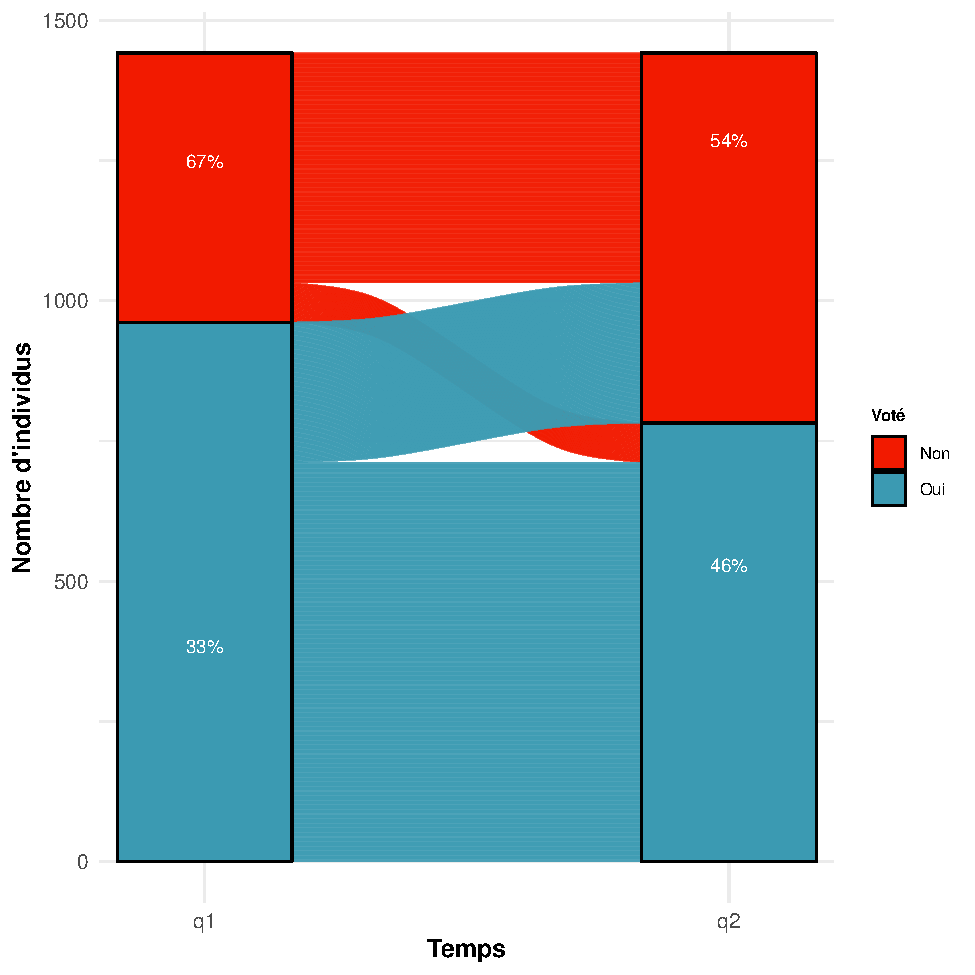
\includegraphics[keepaspectratio]{index_files/figure-pdf/fig-vote_derniers_elections-2020-1.pdf}}

}

\end{minipage}%
%
\begin{minipage}{0.50\linewidth}

\subcaption{\label{fig-vote_derniers_elections-2020-2}Percentages}

\centering{

\pandocbounded{\includegraphics[keepaspectratio]{index_files/figure-pdf/fig-vote_derniers_elections-2020-2.pdf}}

}

\end{minipage}%

\end{figure}%

\subsubsection{Promo 2021-22}\label{promo-2021-22}

\begin{figure}

\caption{\label{fig-vote_derniers_elections-2021}Promo 2021-22. Change
in volunteers reporting whether they voted or not during the last
elections, between Q1 and Q2. Note that this analysis considers only
answers of volunteers who answered either yes or no at \emph{both} time
points.}

\begin{minipage}{0.50\linewidth}

\subcaption{\label{fig-vote_derniers_elections-2021-1}Alluvial plot}

\centering{

\pandocbounded{\includegraphics[keepaspectratio]{index_files/figure-pdf/fig-vote_derniers_elections-2021-1.pdf}}

}

\end{minipage}%
%
\begin{minipage}{0.50\linewidth}

\subcaption{\label{fig-vote_derniers_elections-2021-2}Percentages}

\centering{

\pandocbounded{\includegraphics[keepaspectratio]{index_files/figure-pdf/fig-vote_derniers_elections-2021-2.pdf}}

}

\end{minipage}%

\end{figure}%

\subsubsection{Promo 2022-23}\label{promo-2022-23}

\begin{figure}

\caption{\label{fig-vote_derniers_elections-2022}Promo 2022-23. Change
in volunteers reporting whether they voted or not during the last
elections, between Q1 and Q2. Note that this analysis considers only
answers of volunteers who answered either yes or no at \emph{both} time
points.}

\begin{minipage}{0.50\linewidth}

\subcaption{\label{fig-vote_derniers_elections-2022-1}Alluvial plot}

\centering{

\pandocbounded{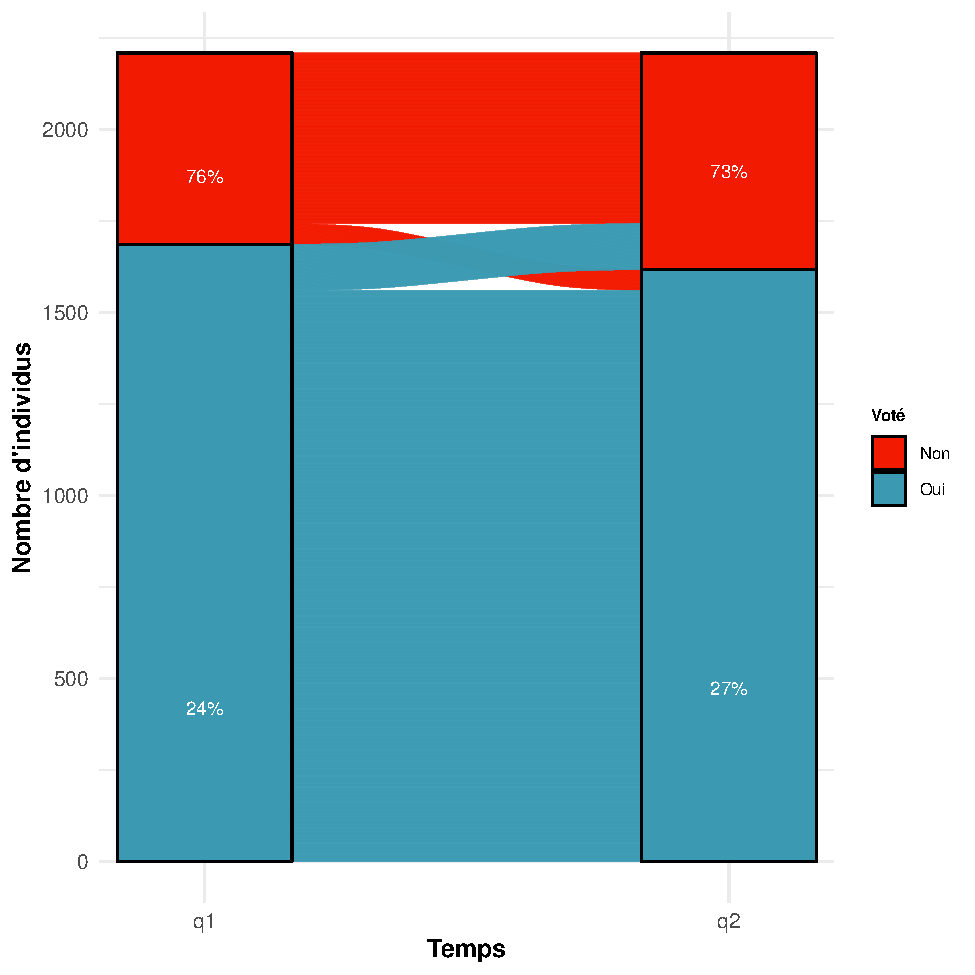
\includegraphics[keepaspectratio]{index_files/figure-pdf/fig-vote_derniers_elections-2022-1.pdf}}

}

\end{minipage}%
%
\begin{minipage}{0.50\linewidth}

\subcaption{\label{fig-vote_derniers_elections-2022-2}Percentages}

\centering{

\pandocbounded{\includegraphics[keepaspectratio]{index_files/figure-pdf/fig-vote_derniers_elections-2022-2.pdf}}

}

\end{minipage}%

\end{figure}%

\subsubsection{Promo 2023-24}\label{promo-2023-24}

\begin{figure}

\caption{\label{fig-vote_derniers_elections-2023}Promo 2023-24. Change
in volunteers reporting whether they voted or not during the last
elections, between Q1 and Q2. Note that this analysis considers only
answers of volunteers who answered either yes or no at \emph{both} time
points.}

\begin{minipage}{0.50\linewidth}

\subcaption{\label{fig-vote_derniers_elections-2023-1}Alluvial plot}

\centering{

\pandocbounded{\includegraphics[keepaspectratio]{index_files/figure-pdf/fig-vote_derniers_elections-2023-1.pdf}}

}

\end{minipage}%
%
\begin{minipage}{0.50\linewidth}

\subcaption{\label{fig-vote_derniers_elections-2023-2}Percentages}

\centering{

\pandocbounded{\includegraphics[keepaspectratio]{index_files/figure-pdf/fig-vote_derniers_elections-2023-2.pdf}}

}

\end{minipage}%

\end{figure}%

\subsection{Acting for society}\label{acting-for-society}

The figures in this section show changes in volunteers perception on
whether their individual action can contribute to changing society, for
the different promos (promo 2020-21,
Figure~\ref{fig-action_individuelle_societe-2020}; promo 2021-22,
Figure~\ref{fig-vote_derniers_elections-2021}; 2022-23,
Figure~\ref{fig-vote_derniers_elections-2022}; 2023-24,
Figure~\ref{fig-vote_derniers_elections-2023})\footnote{Note that for
  the promo 2023-24, q3 is not yet available, and therefore the promo
  cannot be inclueded here}. Descriptively, there is no clear positive
or negative trend either.

\subsubsection{Promo 2020-21}\label{promo-2020-21-1}

\begin{figure}

\caption{\label{fig-action_individuelle_societe-2020}Promo 2020-21.
Change in volunteers reporting whether they think their individual
action can contribute to changing society, between Q1 and Q2. Note that
this analysis considers only answers of volunteers who answered at
\emph{both} time points.}

\begin{minipage}{0.50\linewidth}

\subcaption{\label{fig-action_individuelle_societe-2020-1}Alluvial plot}

\centering{

\pandocbounded{\includegraphics[keepaspectratio]{index_files/figure-pdf/fig-action_individuelle_societe-2020-1.pdf}}

}

\end{minipage}%
%
\begin{minipage}{0.50\linewidth}

\subcaption{\label{fig-action_individuelle_societe-2020-2}Percentages}

\centering{

\pandocbounded{\includegraphics[keepaspectratio]{index_files/figure-pdf/fig-action_individuelle_societe-2020-2.pdf}}

}

\end{minipage}%

\end{figure}%

\subsubsection{Promo 2021-22}\label{promo-2021-22-1}

\begin{figure}

\caption{\label{fig-action_individuelle_societe-2021}Promo 2021-22.
Change in volunteers reporting whether they think their individual
action can contribute to changing society, between Q1 and Q2. Note that
this analysis considers only answers of volunteers who answered at
\emph{both} time points.}

\begin{minipage}{0.50\linewidth}

\subcaption{\label{fig-action_individuelle_societe-2021-1}Alluvial plot}

\centering{

\pandocbounded{\includegraphics[keepaspectratio]{index_files/figure-pdf/fig-action_individuelle_societe-2021-1.pdf}}

}

\end{minipage}%
%
\begin{minipage}{0.50\linewidth}

\subcaption{\label{fig-action_individuelle_societe-2021-2}Percentages}

\centering{

\pandocbounded{\includegraphics[keepaspectratio]{index_files/figure-pdf/fig-action_individuelle_societe-2021-2.pdf}}

}

\end{minipage}%

\end{figure}%

\subsubsection{Promo 2022-23}\label{promo-2022-23-1}

\begin{figure}

\caption{\label{fig-action_individuelle_societe-2022}Promo 2022-23.
Change in volunteers reporting whether they think their individual
action can contribute to changing society, between Q1 and Q2. Note that
this analysis considers only answers of volunteers who answered at
\emph{both} time points.}

\begin{minipage}{0.50\linewidth}

\subcaption{\label{fig-action_individuelle_societe-2022-1}Alluvial plot}

\centering{

\pandocbounded{\includegraphics[keepaspectratio]{index_files/figure-pdf/fig-action_individuelle_societe-2022-1.pdf}}

}

\end{minipage}%
%
\begin{minipage}{0.50\linewidth}

\subcaption{\label{fig-action_individuelle_societe-2022-2}Percentages}

\centering{

\pandocbounded{\includegraphics[keepaspectratio]{index_files/figure-pdf/fig-action_individuelle_societe-2022-2.pdf}}

}

\end{minipage}%

\end{figure}%

\section{Are there trends between different cohorts of
volunteers?}\label{sec-between-change}

There are many possible differences to investigate between cohorts.
Here, we report XX {[}add two other variables{]}.

\subsection{Satisfaction}\label{satisfaction}

Figure~\ref{fig-satisfaction} shows how different cohorts evaluated
their satisfaction with the service civique.

\begin{figure}

\caption{\label{fig-satisfaction}Satisfaction between cohorts.}

\centering{

\pandocbounded{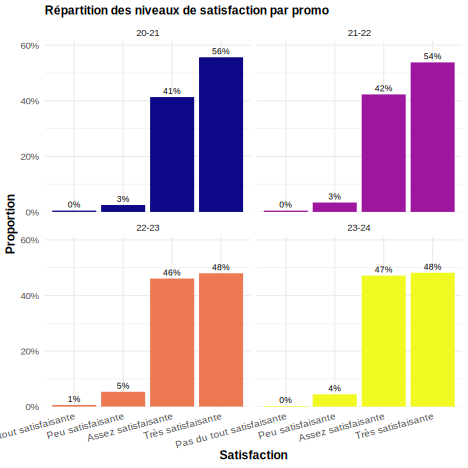
\includegraphics[keepaspectratio]{index_files/figure-pdf/fig-satisfaction-1.pdf}}

}

\end{figure}%

\section{Predictions}\label{predictions}

Note that all predictions here are just statistical associations--they
tell us about differences we observe, but they do not provide proof for
causal conclusions on why we observe these differences.

\subsection{What predicts whether volunteers end their contract early
(rupture)?}\label{sec-rupture}

Figure~\ref{fig-rupture} shows how many volunteers have ended their
contract early (rupture), for the different promos.
Figure~\ref{fig-rupture-motive} provides an overview of the different
reasons, pooling all promos.

\begin{figure}

\caption{\label{fig-rupture}Number of volunteers with a rupture (for
various possible reasons, including positive ones, such as obtaining a
work contract).}

\begin{minipage}{0.50\linewidth}

\subcaption{\label{fig-rupture-1}(absolute numbers)}

\centering{

\pandocbounded{\includegraphics[keepaspectratio]{index_files/figure-pdf/fig-rupture-1.pdf}}

}

\end{minipage}%
%
\begin{minipage}{0.50\linewidth}

\subcaption{\label{fig-rupture-2}(percentages)}

\centering{

\pandocbounded{\includegraphics[keepaspectratio]{index_files/figure-pdf/fig-rupture-2.pdf}}

}

\end{minipage}%

\end{figure}%

\begin{figure}

\caption{\label{fig-rupture-motive}Prevalence of different rupture
motives}

\centering{

\pandocbounded{\includegraphics[keepaspectratio]{index_files/figure-pdf/fig-rupture-motive-1.pdf}}

}

\end{figure}%

Not all volunteers work until the end of their contract. In fact, 22.9\%
of volunteers have a ``rupture'', i.e.~terminate the contract early.
There are various motives for ending one's contract early (see
Table~\ref{tbl-rupture}). Not all of them are necessarily bad,
e.g.~``Embauche en CDD d'au moins 6 mois ou CDI'', and some are outside
of the influence of the volunteers, e.g.~``Fin de validité du Titre de
Séjour''. For our analyses, we focus only on volunteers who ended their
contract early for apparently negative reasons.

To see whether there are differences in different groups, we ran
separate logistic regressions for a selection of variables. The results
are shown in Figure~\ref{fig-rupture-model}. Because the magnitude of
the odds ratios (OR) are not straightforward to interpret,
Figure~\ref{fig-rupture-descriptive} shows descriptive differences in
contract terminations for some groups.

\begin{table}

{\caption{{Different motives for ``rupture'' and whether they were coded
as negative, positive, or external reasons.}{\label{tbl-rupture}}}}

\begin{tabular}[t]{l|l|r}
\hline
motif\_rupture & rupture\_valence & n\\
\hline
01 - Abandon de poste & negative & 1444\\
\hline
02 - Faute grave d'une des parties & negative & 455\\
\hline
03 - Force majeure & negative & 280\\
\hline
04 - Embauche en CDD d'au moins 6 mois ou CDI & positive & 621\\
\hline
05 - Embauche en CDD moins de 6 mois & positive & 383\\
\hline
06 - Commun accord entre les parties & negative & 2761\\
\hline
07 - Le volontaire n'a jamais pris son poste & negative & 13\\
\hline
08 - Retrait de l'agrément de la structure d'accueil & negative & 3\\
\hline
09 - Reprise d'études & positive & 412\\
\hline
10 - Fin de validité du Titre de Séjour & raisons externes & 39\\
\hline
NA & NA & 21549\\
\hline
\end{tabular}

\end{table}

\begin{figure}

\caption{\label{fig-rupture-model}Effects of demographic factors on
negative rupture. Coefficients are the results of separate logistic
regressions for each variable. For categorical variables, a baseline has
been chosen in the model (refer to the codebook to see the omitted
baseline category). Each bar or dot in the chart shows how a factor
(like age, gender, or education) relates to the chance of a rupture. An
odds ratio of 1 means that this group has the same chance of a rupture
as the baseline group. More than 1 means that this group is more likely
to have a rupture. For example, an odds ratio of 2.0 means twice as
likely. Less than 1 means that this group is less likely to have a
rupture. An odds ratio of 0.5 means half as likely. The lines show
uncertainty (confidence intervals). If they cross 1, the difference
might not be meaningful (in this case, the result is not statistically
significant). The logarithmic scale is used so that in the visualization
for the positive and negative odds ratio's to be symmetric (i.e.~that 2
is as far away from 1 as is 0.5).}

\centering{

\pandocbounded{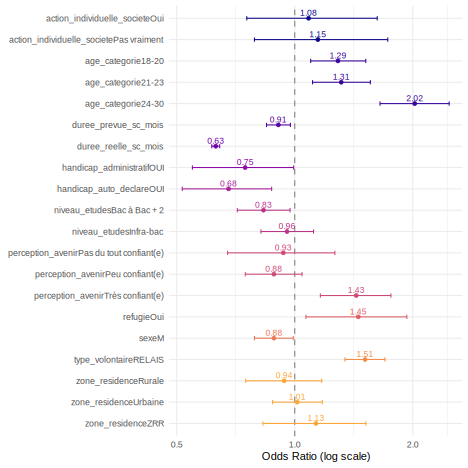
\includegraphics[keepaspectratio]{index_files/figure-pdf/fig-rupture-model-1.pdf}}

}

\end{figure}%

\begin{figure}

\caption{\label{fig-rupture-descriptive}Percentages of rupture for
(allegedly) negative reasons for different groups, for different
variables.}

\centering{

\pandocbounded{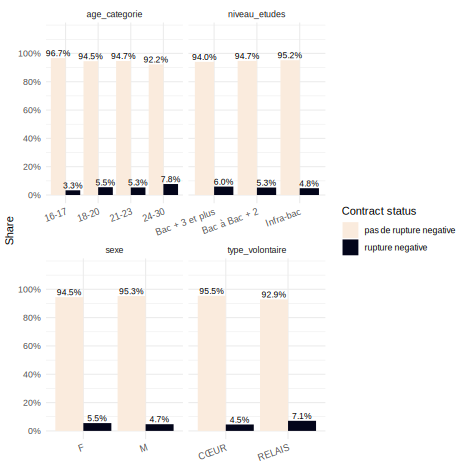
\includegraphics[keepaspectratio]{index_files/figure-pdf/fig-rupture-descriptive-1.pdf}}

}

\end{figure}%

How to make sense of the odds ratios? Take the example of the type of
volunteers (\texttt{type\_volontaire}). Table~\ref{tbl-OR-example} shows
the count, odds and share for rupture vs.~no rupture for a negative
motive.

\begin{table}

{\caption{{Count, odds and share for rupture vs.~no rupture for a
negative motive, according to which type of
volunteer.}{\label{tbl-OR-example}}}}

\begin{tabular}[t]{l|r|r|r|r}
\hline
type\_volontaire & pas de rupture negative & rupture negative & odds & share\\
\hline
CŒUR & 19863 & 945 & 21.019 & 0.045\\
\hline
RELAIS & 6642 & 510 & 13.024 & 0.071\\
\hline
\end{tabular}

\end{table}

In this case the OR is odds of ``CŒUR'' divided by odds of ``RELAIS''
(OR = 1.6138667).

For non-demographic variables, investigating their relationship with
rupture is not possible--simply because, by definition, for questions
that have been only asked at ``q2'' and ``q3'', volunteers who had ended
their contract early were not available anymore (see
Table~\ref{tbl-rupture-candidates}). Only for the two variables that
have been asked at ``q1'' (\texttt{perception\_avenir} and
\texttt{action\_individuelle\_societe}) we can look at their
relationship with rupture (Figure~\ref{fig-rupture-model}).

\begin{table}

{\caption{{Candidate variables to evaluating their association with
rupture.}{\label{tbl-rupture-candidates}}}}

\begin{tabular}[t]{l|l}
\hline
variable & source\\
\hline
perception\_avenir & q1\\
\hline
action\_individuelle\_societe & q1\\
\hline
projet\_avenir\_concret & q2\\
\hline
comparaison\_utilite\_autres & q2\\
\hline
fierte & q2\\
\hline
confiance\_en\_soi & q2\\
\hline
confiance\_avenir\_personnel & q2\\
\hline
action\_individuelle\_societe & q3\\
\hline
impact\_situation\_actuelle & q3\\
\hline
integration & q2\\
\hline
\end{tabular}

\end{table}

\subsection{What predicts whether volunteers are more satisfied
?}\label{sec-satisfaction}

In this section, we look at satisfaction (``D'une manière générale,
diriez-vous que votre Service Civique s'est déroulé de façon\ldots{}''
with levels 1, ``pas du tout satisfaisainte'', to 4, ``très
satisfaisante'')\footnote{In all analyses we treat this as a continuous
  variable}. As shown in Figure~\ref{fig-satisfaction-descriptive},
taking all cohorts together, the majority of volunteers thinks their
experience is ``très satisfaisant''.

\begin{figure}

\caption{\label{fig-satisfaction-descriptive}Répartition des niveaux de
satisfaction}

\centering{

\pandocbounded{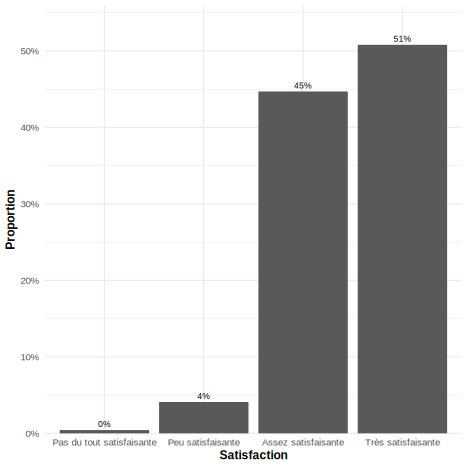
\includegraphics[keepaspectratio]{index_files/figure-pdf/fig-satisfaction-descriptive-1.pdf}}

}

\end{figure}%

To see whether there are statistical differences between different
categories of volunteers, we ran separate regression models for a
selection of variables. The results are shown in
Figure~\ref{fig-satisfaction-demographic-variables}, for demographic
variables, and Figure~\ref{fig-satisfaction-other-variables}, for other
variables. The estimates in these figures are the results of separate
linear regressions for each variable. All likert scale type responses
(such as satisfaction) have been coded as numeric (from 1 to 4). How to
interpret the coefficients? For categorical variables, a baseline has
been chosen in the model (refer to the codebook to see the omitted
baseline category). The estimate shown in the graph is how much,
compared to this baseline, satisfaction increases or decreases (on a
scale from 1 to 4). For numeric variables, estimates represent how much
satisfaction increases or decreases after increasing the variable by one
unit.

\begin{figure}

\caption{\label{fig-satisfaction-demographic-variables}Effects of
demographic factors on satisfaction.}

\centering{

\pandocbounded{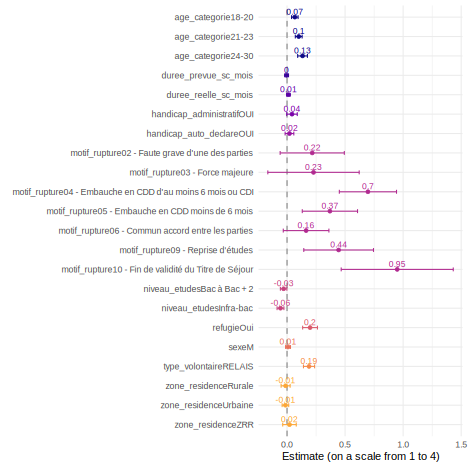
\includegraphics[keepaspectratio]{index_files/figure-pdf/fig-satisfaction-demographic-variables-1.pdf}}

}

\end{figure}%

\begin{figure}

\caption{\label{fig-satisfaction-other-variables}Effects of other,
non-demographic factors on satisfaction.}

\centering{

\pandocbounded{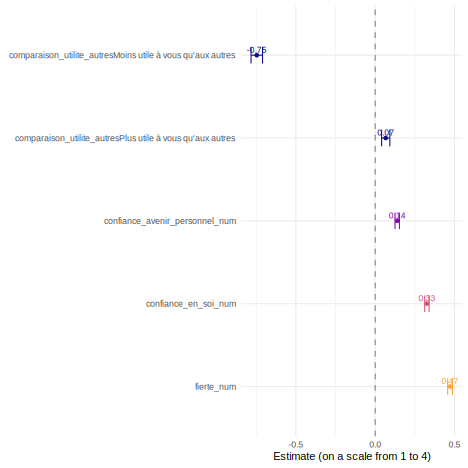
\includegraphics[keepaspectratio]{index_files/figure-pdf/fig-satisfaction-other-variables-1.pdf}}

}

\end{figure}%

\subsection{What predicts whether volunteers are more confident in their
future ?}\label{sec-perception-avenir}

In this section, we look at confidence in one's future (``Concernant
votre avenir, êtes-vous\ldots?'' with levels 1, ``Pas du tout
confiant.e'', to 4, ``Très confiant.e'')\footnote{In all analyses we
  treat this as a continuous variable}. As shown in
Figure~\ref{fig-perception-avenir-descriptive}, taking all cohorts
together, the majority of volunteers are ``assez confiant.e''.

\begin{figure}

\caption{\label{fig-perception-avenir-descriptive}Répartition des
niveaux de satisfaction}

\centering{

\pandocbounded{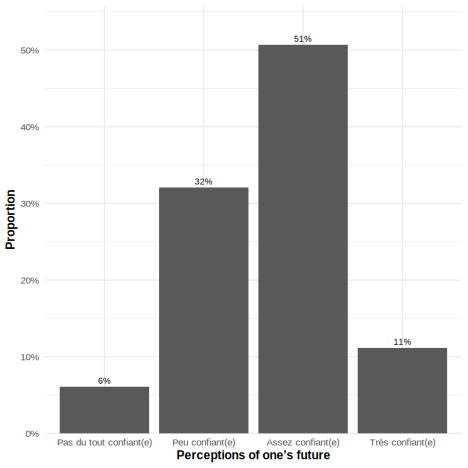
\includegraphics[keepaspectratio]{index_files/figure-pdf/fig-perception-avenir-descriptive-1.pdf}}

}

\end{figure}%

To see whether there are statistical differences between different
categories of volunteers, we ran separate regression models for a
selection of variables. The results are shown in
Figure~\ref{fig-satisfaction-demographic-variables}, for demographic
variables, and Figure~\ref{fig-satisfaction-other-variables}, for other
variables. The estimates in these figures are the results of separate
linear regressions for each variable. All likert scale type responses
(such as satisfaction) have been coded as numeric (from 1 to 4). How to
interpret the coefficients? For categorical variables, a baseline has
been chosen in the model (refer to the codebook to see the omitted
baseline category). The estimate shown in the graph is how much,
compared to this baseline, satisfaction increases or decreases (on a
scale from 1 to 4). For numeric variables, estimates represent how much
satisfaction increases or decreases after increasing the variable by one
unit.

\begin{figure}

\caption{\label{fig-perception-avenir-demographic-variables}Effects of
demographic factors on confidence in one's future.}

\centering{

\pandocbounded{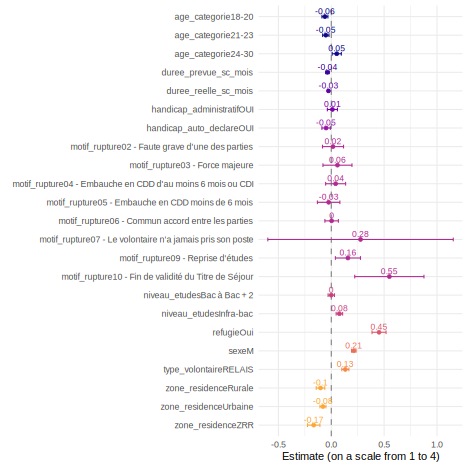
\includegraphics[keepaspectratio]{index_files/figure-pdf/fig-perception-avenir-demographic-variables-1.pdf}}

}

\end{figure}%

\begin{figure}

\caption{\label{fig-perception-avenir-other-variables}Effects of other,
non-demographic factors on confidence in one's future.}

\centering{

\pandocbounded{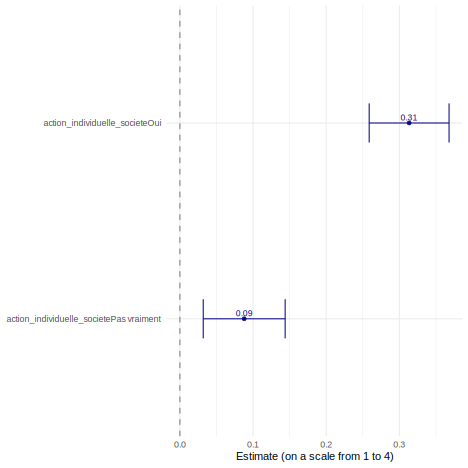
\includegraphics[keepaspectratio]{index_files/figure-pdf/fig-perception-avenir-other-variables-1.pdf}}

}

\end{figure}%

\section{Differences between
programs}\label{differences-between-programs}

\subsection{Ciné}\label{sec-cine}

Volunteers who work in cine-related projects tend to be older and more
educated. Refugies are less likely to be cine volunteers. If there is a
preliminary end to the contract, cine volunteers are more likely to do
so because they were offered a CDD of less than 6 months. Refugees are
less likely to be cine volunteers, and women, as well as people from
urban areas are more likely.

\begin{figure}

\caption{\label{fig-cine-demographic-variables}Differences in
Ciné-related vs.~other programs along demographic factors}

\centering{

\pandocbounded{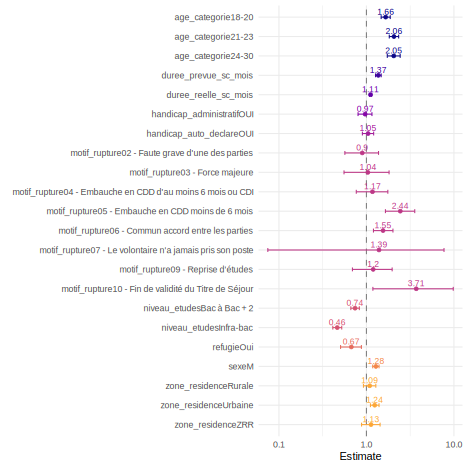
\includegraphics[keepaspectratio]{index_files/figure-pdf/fig-cine-demographic-variables-1.pdf}}

}

\end{figure}%

\subsection{Ecovolonterre}\label{sec-ecovolonterre}

Ecovolonterres tend to be older (mostly in the 21 to 23 agegroup) and
more educated than other volunteers. They tend to plan for longer
volunteer programs. Ecovolonterres tend to be from more rural but also
urban ares (compared to QVP).

\begin{figure}

\caption{\label{fig-ecovolonterre-demographic-variables}Differences in
Ecovolonterre vs.~other programs along demographic factors}

\centering{

\pandocbounded{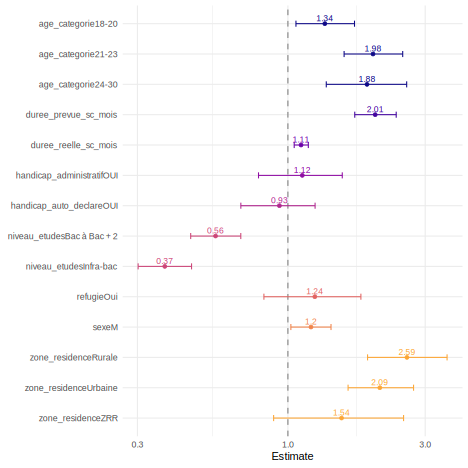
\includegraphics[keepaspectratio]{index_files/figure-pdf/fig-ecovolonterre-demographic-variables-1.pdf}}

}

\end{figure}%






\end{document}
